\section{Complete Mission1 Comparisons}
\label{app:extended}
The following generated tables preserve the complete cap sweep behind the focused
main-text comparisons. Event denominators remain the same 11 Mission1 validation
anomalies. Costs are actual encoded MiB under shared caps, not matched expenditure.
Repeated arms, caps, and receiver ranks are not independent faults.

\begin{table}[htbp]
\centering\footnotesize
% Generated native validation pilot; development results only.
\begin{tabular}{rlrrrr}
\toprule
Cap & Policy & MiB & Raw events & Level & PCA \\
\midrule
256 & Uniform & 6.22 & 4/11 & 4/11 & 4/11 \\
256 & Summaries & 5.62 & 0/11 & -- & -- \\
256 & Threshold & 0.81 & 10/11 & 10/11 & 10/11 \\
256 & Adaptive & 2.63 & 11/11 & 11/11 & 10/11 \\
512 & Uniform & 12.54 & 5/11 & 5/11 & 5/11 \\
512 & Summaries & 12.04 & 0/11 & -- & -- \\
512 & Threshold & 0.81 & 10/11 & 10/11 & 10/11 \\
512 & Adaptive & 3.57 & 11/11 & 11/11 & 10/11 \\
1024 & Uniform & 25.04 & 5/11 & 5/11 & 5/11 \\
1024 & Summaries & 24.88 & 0/11 & -- & -- \\
1024 & Threshold & 0.81 & 10/11 & 10/11 & 10/11 \\
1024 & Adaptive & 6.30 & 11/11 & 11/11 & 11/11 \\
2048 & Uniform & 50.62 & 4/11 & 4/11 & 4/11 \\
2048 & Summaries & 50.17 & 0/11 & -- & -- \\
2048 & Threshold & 0.81 & 10/11 & 10/11 & 10/11 \\
2048 & Adaptive & 11.69 & 11/11 & 11/11 & 11/11 \\
\bottomrule
\end{tabular}

\caption{Original four-policy, four-cap native pilot. Summary bounds are coarse
bucket evidence and do not supply raw-input receiver events.}
\label{tab:native-complete}
\end{table}

\begin{table}[htbp]
\centering\footnotesize
% Generated randomized validation comparison; seed ranges are not event confidence intervals.
\begin{tabular}{rlrrr}
\toprule
Cap & Policy & Mean MiB & PCA events: mean [range] & Context (\%) \\
\midrule
256 & Reservoir & 6.22 & 3.9 [3, 5] & 4.8 \\
256 & Random phase & 6.20 & 4.0 [3, 5] & 4.7 \\
512 & Reservoir & 12.54 & 4.6 [3, 6] & 11.7 \\
512 & Random phase & 12.49 & 4.8 [3, 6] & 11.0 \\
1024 & Reservoir & 25.15 & 5.1 [4, 7] & 23.8 \\
1024 & Random phase & 24.96 & 5.4 [4, 8] & 21.8 \\
2048 & Reservoir & 50.67 & 7.0 [5, 9] & 50.6 \\
2048 & Random phase & 50.44 & 6.7 [5, 9] & 45.9 \\
\bottomrule
\end{tabular}

\caption{All four caps for the seeded controls. Ranges are observed seed minima
and maxima on the same events, not generalization confidence intervals.}
\label{tab:seeded-complete}
\end{table}

\begin{table}[htbp]
\centering\small
% Generated paired development ablations; caps are not equal expenditures.
\begin{tabular}{rlrrr}
\toprule
Cap & Variant & MiB & PCA events & Pre-context (\%) \\
\midrule
256 & Full & 2.63 & 10/11 & 24.2 \\
256 & No pre & 2.63 & 10/11 & 0.0 \\
256 & No post & 2.63 & 10/11 & 24.2 \\
256 & No background & 0.84 & 10/11 & 41.5 \\
512 & Full & 3.57 & 10/11 & 64.3 \\
512 & No pre & 3.55 & 10/11 & 1.8 \\
512 & No post & 3.56 & 10/11 & 64.3 \\
512 & No background & 0.88 & 10/11 & 64.3 \\
1024 & Full & 6.30 & 11/11 & 64.3 \\
1024 & No pre & 6.26 & 11/11 & 1.8 \\
1024 & No post & 6.28 & 11/11 & 64.3 \\
1024 & No background & 0.90 & 10/11 & 64.3 \\
2048 & Full & 11.69 & 11/11 & 67.1 \\
2048 & No pre & 11.66 & 11/11 & 9.1 \\
2048 & No post & 11.68 & 11/11 & 67.1 \\
2048 & No background & 0.90 & 10/11 & 64.3 \\
\bottomrule
\end{tabular}

\caption{Paired single-component removals. No-background releases its reserved
quota to trigger/context capture. Full arms match the original packet bytes.}
\label{tab:ablation-complete}
\end{table}

\begin{table}[htbp]
\centering\scriptsize
% Generated from completed receiver mismatch benchmark.
\begin{tabular}{llrrrr}
\toprule
Capture & Policy & MiB & PCA events & Blind kept/available & Pre-context (\%) \\
\midrule
Difference & Threshold & 0.81 & 10/11 & 0/1 & 0.0 \\
Difference & Adaptive & 6.30 & 11/11 & 1/1 & 64.3 \\
Difference & Coverage & 6.30 & 11/11 & 1/1 & 66.3 \\
Level & Threshold & 1.38 & 10/11 & 0/1 & 0.0 \\
Level & Adaptive & 6.67 & 11/11 & 1/1 & 65.1 \\
Level & Coverage & 6.67 & 11/11 & 1/1 & 67.1 \\
PCA & Threshold & 1.58 & 11/11 & 0/0 & 0.0 \\
PCA & Adaptive & 8.86 & 11/11 & 0/0 & 65.1 \\
PCA & Coverage & 8.75 & 11/11 & 0/0 & 66.3 \\
Disabled & Threshold & 0.80 & 0/11 & 0/11 & 0.0 \\
Disabled & Adaptive & 6.22 & 4/11 & 4/11 & 1.8 \\
Disabled & Coverage & 6.22 & 6/11 & 6/11 & 2.9 \\
\bottomrule
\end{tabular}

\caption{The 1,024-byte capture mismatch matrix. Blind-event counts refer to
within-event trigger crossings and receiver-specific full-archive support; nearby
triggers may still retain event samples as context.}
\label{tab:mismatch-complete}
\end{table}

\begin{table}[htbp]
\centering\small
% Generated finite-buffer delivery comparison.
\begin{tabular}{llrrr}
\toprule
Policy & Link & Wire MiB & Delivered packets & PCA events \\
\midrule
Uniform & Ample & 28.24 & 26304/26304 & 5/11 \\
Uniform & Congested & 8.56 & 4498/26304 & 4/11 \\
Uniform & Lossy & 28.24 & 23638/26304 & 5/11 \\
Adaptive & Ample & 7.11 & 26304/26304 & 11/11 \\
Adaptive & Congested & 7.04 & 26182/26304 & 11/11 \\
Adaptive & Lossy & 7.11 & 23638/26304 & 10/11 \\
Coverage & Ample & 7.11 & 26304/26304 & 11/11 \\
Coverage & Congested & 7.04 & 26182/26304 & 11/11 \\
Coverage & Lossy & 7.11 & 23638/26304 & 10/11 \\
\bottomrule
\end{tabular}

\caption{Illustrative delivery at the 1,024-byte recording cap. Wire expenditure
includes overhead and unsuccessful or partial transmissions.}
\label{tab:delivery-complete}
\end{table}

\begin{figure}[htbp]
\centering
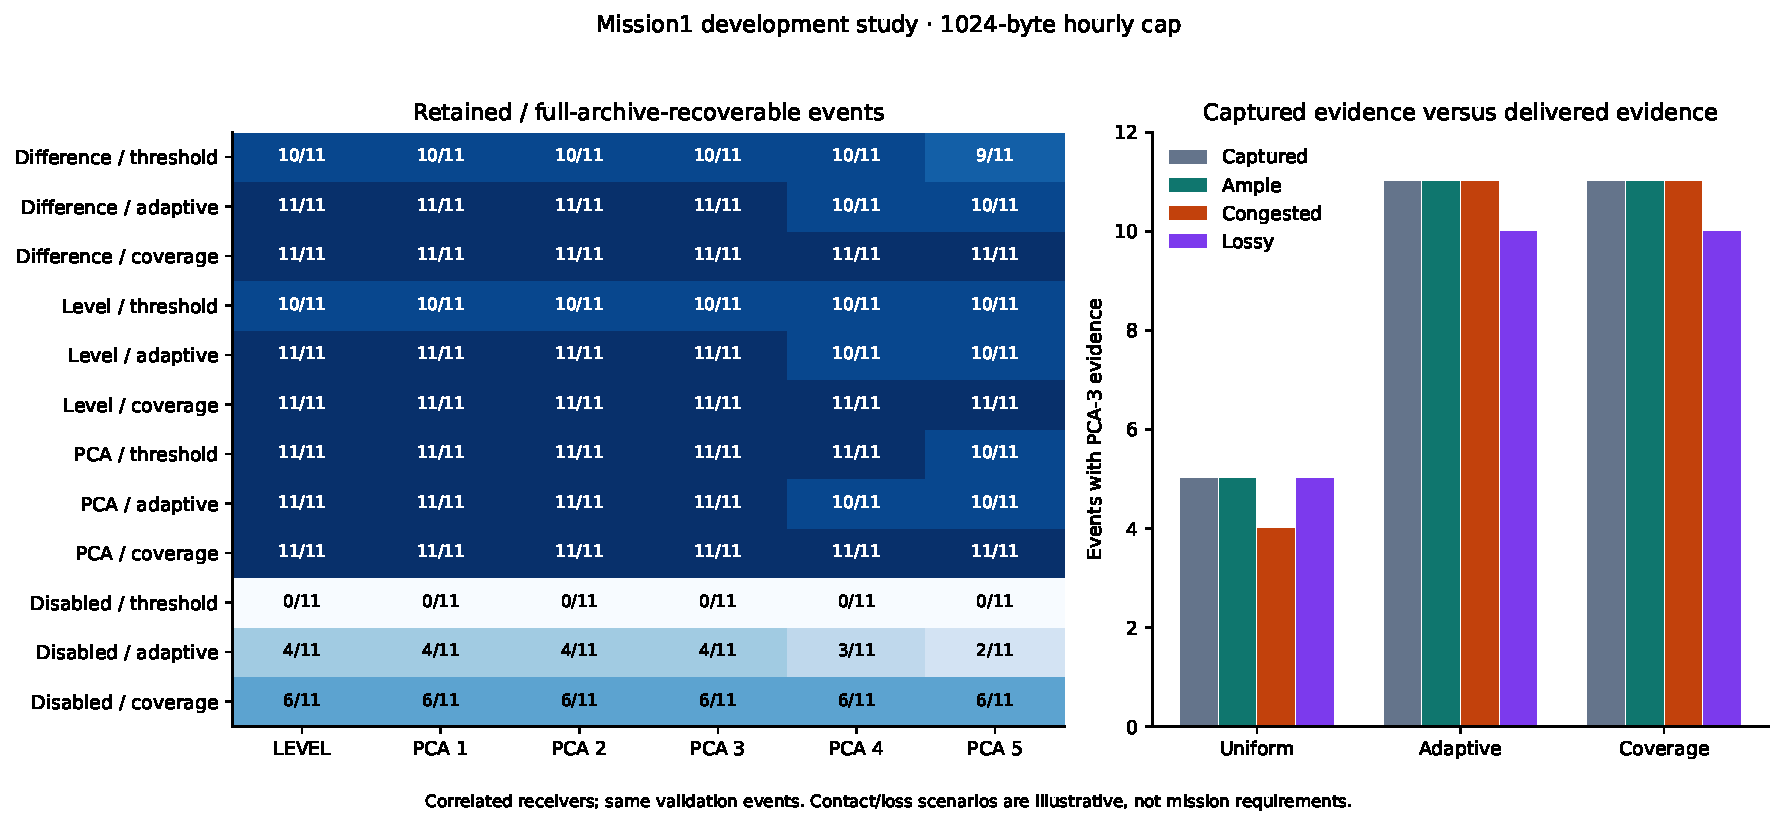
\includegraphics[width=\linewidth]{generated/receiver_mismatch.pdf}
\caption{Mission1 pointwise receiver sensitivity and illustrative delivery.
Correlated ranks and shared events restrict inference. These plotted counts do
not constitute validation against independent future detector families.}
\label{fig:mismatch-complete}
\end{figure}
